\newpage
\section{Cryptomining basics} \label{toc:grundlagenkryptomining}

\acused{SHA}

This chapter lays the foundations for understanding the term "cryptomining". After this part, the reader should
have a picture of what mining is and why, in the blockchain domain, mining is a fundamental process. Furthermore
he should be able to understand the basic structure of an enterprise data center that is exclusively mining.
To achieve this, the first step in chapter \ref{toc:kryptowaehrungenundblockchain} is to give a brief
introduction to the blockchain and its basic structure. There, it is established why the principle of
mining was introduced and what it is used for. In the chapter \ref{toc:miningundkonsensalgorithmen}, the process of
of the mining is dealt with. The basic functioning and necessity of mining is shown. After
these basics are laid, the operation of a mining data center is described. The understanding of
data centers that specialize in mining is important for the rest of the paper, as they are to be optimized from a financial perspective.
For this purpose, the basic structure of such a data center of the Genesis Group is exemplarily
described. It is shown which \acp{KPI} of these data centers are important. These are used to optimize the
data centers to be able to optimize them financially. All this is discussed in chapter \ref{toc:miningrechenzentren}. Following
this knowledge is then used to identify possible starting points for a business intelligence system
and to model an exemplary process at the end of the thesis.

\subsection{Basic technologies} \label{toc:technologie}

The concept of blockchain was first described in 2008 in a whitepaper using the example of Bitcoin,
published by the pseudonym Satoshi Nakamoto.\footcite[Cf.][]{nakamoto2008bitcoin} Many companies and start-ups in
a wide variety of industries are looking at blockchain-based
systems, such as in the financial industry, in the information sector, but also in the health care and
transport sectors.\footcite[Cf.][Chap. 4.1]{friedlmaier2018disrupting} Another branch that has emerged through the introduction of
cryptocurrencies are companies that specialize in mining cryptocurrencies. To understand the
technical basis for this business case, the following two subsections describe what
a blockchain is and what characteristics make mining necessary. How mining is technologically implemented and why
it provides a way to make money is described in chapter \ref{toc:miningundkonsensalgorithmen}.

\subsubsection{Definition of Blockchain} \label{toc:kryptowaehrungenundblockchain}

A blockchain, as the name translates, is a chain of blocks. Through the use of cryptographic
processes, data on a blockchain is subsequently stored immutably, which can make this technology attractive for many
applications.\footcite[Cf.][p. 1]{friedlmaier2018disrupting} The atomic unit of a blockchain
is a single block. In the case of Bitcoin, this consists of two different parts: a list of transactions
and the so-called "block header", which contains the most important meta-information and properties of the block.\footcite[Cf.][p. 48]{bhaskar2015bitcoin}\footcite[Cf.][p. 4]{nakamoto2008bitcoin}

\begin{figure}[H]
    \caption{Structure of a single block}
    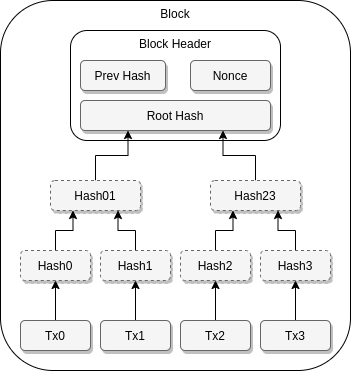
\includegraphics[width=0.4\textwidth]{blockstructure}
    \label{figure:blockstructure}
    \\
    \cite[Source: Based on][p. 4]{nakamoto2008bitcoin}
\end{figure}

The following is a list of the elementary parameters that can be found in a block header
(Cf. Fig. \ref{figure:blockstructure}):

\begin{itemize}
    \item \textbf{Previous block hash: }Because the blocks are arranged into a logical chain, there must be some way
    to identify the order in which the blocks are written. This is achieved similar to a
    chained list by calculating a hash from the block header of the previous block by applying the \ac{SHA}256
    hash function and entering it into the field "Previous block hash".\footcite[Cf.][p. 4]{nakamoto2008bitcoin} This achieves,
    that the sequence of blocks in the blockchain is well-defined back to the first block ("Genesis Block")\footcite[Cf.][Fig. 3.2]{bhaskar2015bitcoin}
    and is traceable (Cf. Fig. \ref{figure:blockchainstructure}).
    Subsequent modification of a block will cause the chain to break, as this will change the hash value of the
    tampered block.
    \item \textbf{Merkle Root: }This field is used to enter the result of the Merkle tree, which is calculated from all transactions.\footcite[Cf.][p. 4]{nakamoto2008bitcoin}
    This is also a hash value. A hash value is formed from
    each individual transaction and merged into a hash value via a binary tree. This value is called
    "Merkle Root" (cf. \ref{figure:blockstructure}). This allows the integrity of each transaction
    which is located in this block. A subsequent change is no longer possible, because in this case,
    the hash value of the Merkle root in the block header and thus the resulting hash of the block header would change.
    Consequently, the chain would break in this case and the blockchain would be destroyed.
    \item \textbf{Nonce: }This is a random number used to generate a hash of the block header,
    which is subject to certain constraints.\footcite[Cf.][p. 745]{mukhopadhyay2016brief}\footcite[Cf.][p. 136]{courtois2014optimizing}
    Guessing and verifying this value is called mining.\footcite[Cf.][pp. 50]{bhaskar2015bitcoin}\footcite[Cf.][p. 24]{han2019demystifying}
    How this value is found and what rules it must obey is described in chapter \ref{toc:miningundkonsensalgorithmen}
    described.
\end{itemize}

\begin{figure}[H]
    \caption{Schematic structure of the blockchain}
    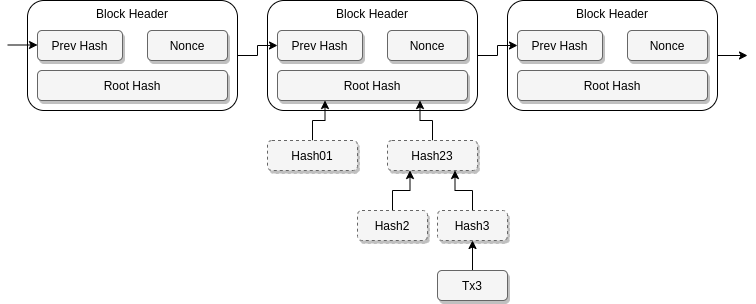
\includegraphics[width=0.8\textwidth]{blockchainstructure}
    \label{figure:blockchainstructure}
    \\
    \cite[Source: Based on][p. 5]{nakamoto2008bitcoin}
\end{figure}

The rest of the block, which in the case of Bitcoin is limited to the size of 1MB, is filled with the corresponding
transactions that have been used to calculate the Merkle root.\footcite[Cf.][p. 746]{mukhopadhyay2016brief}
In general, any data can be stored on a blockchain. There are no restrictions that
it must be transaction data of a currency.

Now there are still two ways to change or delete the data on a blockchain. One case
is the manual deletion of the blockchain. To prevent this, a blockchain is stored in a decentralized manner on many
devices.\footcite[Cf.][p. 46]{bhaskar2015bitcoin} Each of these devices contains a current and correct copy
of the blockchain with all of its data. Such a device is called a "node". Any person in the world can inpect the blockchain, in the case of
Bitcoin, because the data of the Bitcoin Blockchain is publicly available and therefore it is a so-called "permissionless blockchain".\footcite[Cf.][p. 132]{courtois2014optimizing}
If a participant deletes his node or the node is simply
deletes its node or it simply fails, the blockchain is still available and not deleted due to the decentralized replication.

The other case is the modification of a block and a subsequent complete recalculation of all hash values of this blockchain,
which would again result in a new correct blockchain. However, this would contain falsified data.
To prevent this, mining has been introduced, which is nothing more than a guessing game to find the
correct value of the "nonce" described above. This principle is called \ac{PoW} and will be described in detail in the next chapter.\footcite[Cf.][p. 3]{nakamoto2008bitcoin}

In summary, it can be stated that a blockchain is extremely secure against falsification and deletion of data due to its
strong use of cryptographic processes and its decentralization.
The first obvious use case was the application of the blockchain to introduce a digital and decentralized currency, as Satoshi
Satoshi Nakamoto also proposed in his white paper.\footcite[Cf.][]{nakamoto2008bitcoin}

\subsubsection{Definition of mining} \label{toc:miningundkonsensalgorithmen}

Building on the last chapter, this chapter deals with the functioning of mining and the underlying consensus algorithms.
This is important for the remainder of the thesis, since it explains the basic structure of mining
and also during the mining process, important parameters such as the "difficulty" play a role in the overall financial assessment of a mining project,
which contribute to an overall financial assessment of a data center.

Based on the problem that the Bitcoin blockchain consists of a decentralized peer-to-peer network, it is necessary to
be asked how a consensus is generated between the participants and how it is ensured
that fraudulent intentions are prevented. The question becomes how all participants together can reach a valid
consensus and thus make the blockchain trustworthy.\footcite[Cf.][Fig. 3]{derks2018chaining}
To answer these questions, we will look at possible consensus algorithms and explore the principle of
of mining is explained on the basis of the \ac{PoW} consensus.

The first consensus algorithm was described in Satoshi Nakamoto's Bitcoin whitepaper and is called
"Proof-of-Work".\footcite[Cf.][p. 3]{nakamoto2008bitcoin} Since it is not optimal in terms of energy consumption, other algorithms have been developed,
that are much more energy efficient.\footcite[Cf.][]{dwcom2021bitcoin} The best known example is \ac{PoS} or also the use of the
"byzantine fault tolerance", which is also known as the "problem of the Byzantine generals" across the blockchain
industry.\footcite[Cf.][p. 2]{friedlmaier2018disrupting}\footcite[Cf.][p. 746]{mukhopadhyay2016brief}
However, since large computational resources are required only for proof-of-work, the following discussion will focus on this algorithm
using the example of Bitcoin.

The process of mining through proof-of-work can be divided into the following steps:\footcite[Cf.][p. 3]{nakamoto2008bitcoin}\footcite[Cf.][p. 51]{li2019blockchain}

\begin{enumerate}
    \item New transactions are sent to all nodes in the network. These are stored in the so-called "mempool",
    a cache of transactions that have not yet been confirmed, and held for the mining process.
    \item Transactions are packaged into a block by the nodes. The transactions with the highest fees,
    which can be freely chosen by the client, are preferentially merged from the mempool into a block.\footcite[Cf.][p. 53]{bhaskar2015bitcoin}
    The sum of the transaction fees of the block is attributed to the miner
    once he finds a valid block.\footcite[Cf.][p. 4]{nakamoto2008bitcoin}
    \item The mining hardware computes a valid proof-of-work for that block, which the nodes provide to the network.
    This is the actual computationally intensive process. Basically, this process is nothing more
    other than a brute-forcing of hash values.\footcite[Cf.][p. 747]{mukhopadhyay2016brief} Only in this way
    it is possible to compute a correct target hash value, since hash functions are surjective. The so called
    "difficulty" is used to determine how many zeros the resulting hash should start with.\footcite[Cf.][p. 57]{bhaskar2015bitcoin}
    In order to find a suitable hash, the nonce is varied and
    for each value of the nonce, the hash value of the block is computed and verified. If it meets the requirements, which are
    specified by the difficulty, a valid \ac{PoW} has been found. On average, this process should take about ten minutes.\footcite[Cf.][p. 748]{mukhopadhyay2016brief}
    Therefore, the relevant performance metric of the mining hardware is called the
    hashrate.\footcite[Cf.][p. 49]{bhaskar2015bitcoin} This describes how many hash values a device can compute in one second.
    If the overall hashrate in the Bitcoin network increases, so does the
    probability that a valid proof-of-work can be found in less than ten minutes. Therefore, the
    Difficulty is adjusted every 2,016 blocks, so that if the overall hashrate of the network is higher, the variation
    of the starting zeros makes it easier or more difficult to find a valid proof-of-work (Cf.
    Fig. \ref{figure:evolutiondifficulty}).\footcite[Cf.][p. 57]{bhaskar2015bitcoin} Since the creation of the blocks
    takes a lot of computational work, individual fraudsters now have no ability to manipulate the blockchain,
    as long as the majority of participants in mining are honest. 
    \item When a proof-of-work is found, it is sent to all nodes in the Bitcoin network.\footcite[Cf.][pp. 3]{nakamoto2008bitcoin}
    For this purpose, the node connected to the mining hardware forms a
    valid nonce with all the other information and sends it to all nodes in the Bitcoin network.
    \item This block is now verified by the remaining nodes. The verification is successful as soon as the majority of
    nodes accept the block and the construction of a new block is started, using the hash value of the found block as the
    block is used as the previous hash for the new block.\footcite[Cf.][pp. 3]{nakamoto2008bitcoin}
    The operator of the mining hardware receives as a reward the sum of all transaction fees of the block and
    a fixed amount, which is currently 6.25 \ac{BTC} per block.\footcite[Cf.][p. 4]{nakamoto2008bitcoin}\footcite[Cf.][]{btcecho2021halving}\footcite[Cf.][p. 59]{taylor2017evolution}
    The 6.25 \ac{BTC} is called a "block reward." This was initially 50 \ac{BTC} and is reduced by half every 210,000 blocks.\footcite[Cf.][p. 58]{taylor2017evolution}
    This will provide the Bitcoin network with new and
    fresh currency. Subsequently, the process of mining starts all over again.
\end{enumerate}

\begin{figure}[H]
    \caption{Development of the Difficulty of Bitcoin depending on the used hardware and grid size}
    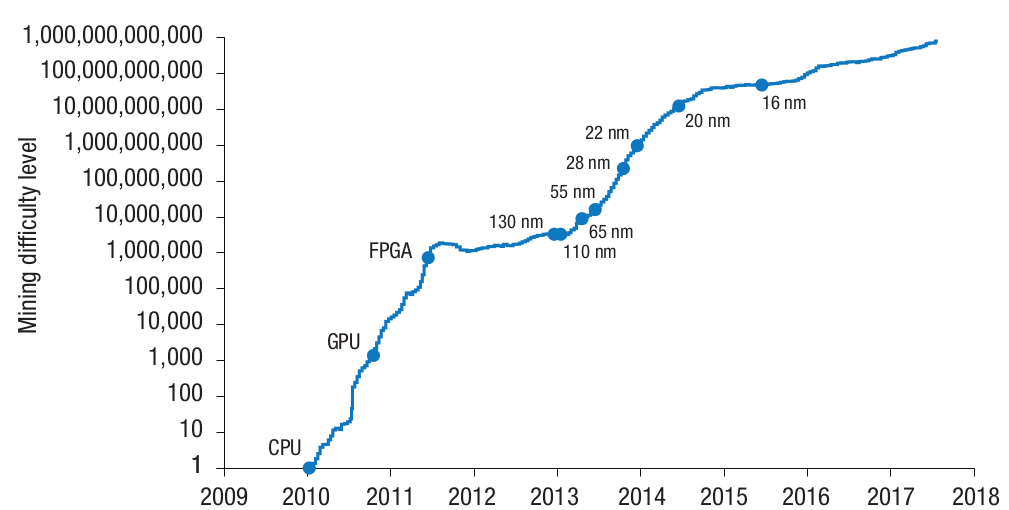
\includegraphics[width=0.8\textwidth]{evolutiondifficulty}
    \label{figure:evolutiondifficulty}
    \\
    \cite[Source: ][Fig. 1b]{taylor2017evolution}
\end{figure}

In principle, the higher your own share of the total hashrate of the network, the higher the probability of successfully finding a block first.
For this reason, operators of mining hardware try to give as much
performance as possible to the network in order to obtain the highest possible payouts. The operation
takes place in relation to the cost of such infrastructure, which is discussed in chap.
\ref{toc:kennzahlenundeinflussfaktoren} in more detail.

Basically, anyone can participate in mining. There are currently three models of how mining can be
done:\footcite[Cf.][p. 53, pp. 57]{bhaskar2015bitcoin}

\begin{itemize}
    \item \textbf{Solo Mining: }This describes the classic method in which participants use their own hardware
    and perform mining. They receive the entire proceeds of a block after a successful proof-of-work.
    \item \textbf{Mining Pools: }In mining pools, the hashrate of many miners is pooled. By pooling the hashrate,
    the probability of finding a valid block is increased. The payout in this
    not the total yield of the block, but rather the percentage of the output that is made available to the mining pool.
    Due to the participation, the individual yields will be lower but more evenly
    turn out. This avoids the risk of not finding a valid proof-of-work for a long time as a solo miner.
    (see Fig. \ref{figure:valuechaindatacenter}).\footcite[Cf.][pp. 58]{bhaskar2015bitcoin}\footcite[Cf.][p. 327]{derks2018chaining}
    \textbf{Mining Contracts: }The third option is to rent mining hardware or purchase a
    hashrate. \footcite[Cf.][pp. 58]{bhaskar2015bitcoin}The proceeds from mining are transferred to the person after deducting the
    contract fees. Consequently, the person does not need to operate his own hardware and can leave this to professional
    companies that can do this much more efficiently than private individuals. Such a product is offered by the
    Genesis Group.
\end{itemize}

\subsection{Mining data centers} \label{toc:miningrechenzentren}

Mining Bitcoins has changed a lot since its introduction in 2009. At that time, hashes were started to be calculated on
normal \acp{CPU}.\footcite[Cf.][pp. 97]{xie2018extreme}\footcite[Cf.][p. 62]{taylor2017evolution}
As explained in chapter \ref{toc:miningundkonsensalgorithmen}, the likelihood of finding a block successfully using proof-of-work
increases with the proportional hashrate to the total network hashrate.
Accordingly, mining hardware operators aim to increase efficiency by reducing the cost per
computed hash. Due to this endeavor, the second generation of mining hardware based on
\acp{GPU} has been developed.\footcite[Cf.][p. 98]{xie2018extreme}\footcite[Cf.][p. 62]{taylor2017evolution}
Due to the evolution of Bitcoin's network hashrate, third-generation hardware based on the
\acp{FPGA} basis.\footcite[Cf.][p. 98]{xie2018extreme}\footcite[Cf.][pp. 62]{taylor2017evolution}
The fourth-generation hardware type is still in use today and is based on
\acp{ASIC}.\footcite[Cf.][pp. 98]{xie2018extreme}\footcite[Cf.][p. 15]{gai2020blockchain} These devices are
specialized by hardware layout to compute hashes highly efficient.{gai2020blockchain}
On the other hand, these chips are not able to compute other things efficiently and thus are only designed for this
specific purpose they were developed. However, there has been a drive not only for higher efficiency, but also
for scaling the mining hardware. In order to maximize the returns from mining, these two drivers have been
combined. This led to the construction of highly specialized ASIC-based data centers dedicated solely to bitcoin mining.\footcite[Cf.][p. 97]{xie2018extreme}
Several such data centers are operated by Genesis Group. These are
described below as examples and their cost and value structure analyzed.

\subsubsection{Structure and operation} \label{toc:aufbauundfunktionsweise}

This chapter describes how a data center that specializes in bitcoin mining is structured
and how it performs mining.

The central component of a mining data center is the mining hardware.\footcite[Cf.][p. 327]{derks2018chaining}
The number of devices operated in such a data center is basically limited only by external factors
such as available space and power supply. In the paper "`Extreme Datacenter Specialization for Planet-Scale.
Computing: ASIC Clouds"', it is described that the devices are usually housed in server racks.\footcite[Cf.][Fig. 5]{xie2018extreme}
This is usually not the case for mining data centers,
as most of the hardware is not built in a 19-inch form factor. Instead, matching heavy-duty racks are
are used, which are placed in rows. Many such rows make up the data center in
itself.\footcite[Cf.][]{appendix:layoutkardok}

As the mining hardware consumes a lot of power, special attention must be paid to the power supply.\footcite[Cf.][p. 327]{derks2018chaining}
The necessary electricity is purchased from external energy companies. The
substations and necessary transformer facilities are located on the outside of the data center or very close by
and ensure a stable power supply. Within the data center, high-voltage sub-distribution boards are
required to supply the individual devices. One of the current models,
the S19 Pro Miner from Bitmain, consumes an average of 3.25kW per device.\footcite[Cf.][]{s19pro2021consumption}
Assuming that there are approximately 12,000 devices in a data center, this results in total
power consumption of 39.0MW for the mining hardware.

In order for the miners to operate stably, the waste heat from the devices must be efficiently removed. For this purpose
a basic structure identical to an ordinary data center consisting of hot and cold aisles is used.
Fans transport cold air into the data center from outside. This warms up as it flows through the
mining hardware, and is carried away through the hot aisle.\footcite[Cf.][]{appendix:layoutkardok} The
electricity costs for cooling make up a significant portion of a mining data center's electricity costs.

In order for the mining hardware to communicate with the blockchain nodes, a network infrastructure is required in addition to the power supply.
This is designed in such a way that each device can communicate with the Internet and thus also with the nodes.
Due to the bandwidth requirements of the internal network, the central
components are dimensioned with a throughput of 10$\frac{Gbit}{s}$. For the peripherals, a data volume of
of 1$\frac{Gbit}{s}$.\footcite[Cf.][]{appendix:networktopology} In order to keep the bandwidth into the internet as small as possible
the mining hardware is connected to a mining proxy, which is installed on an internal server and
and connects to the Bitcoin network and the mining pool used.\footcite[Cf.][]{appendix:miningproxy}
The advantage is that only one connection is needed to an external mining pool.

Finally, control and monitoring software for the mining hardware is installed on additional internal servers.
This software controls and monitors a large number of mining devices.\footnote{https://www.genesis-mining.com/hexa}
The data obtained from the monitoring can be very
interesting for use within business intelligence processes. This evaluation is done
in chapter \ref{toc:ansatzmoeglichkeitenfuerbusinessintelligence}.

\subsubsection{Financial considerations} \label{toc:kennzahlenundeinflussfaktoren}

In diesem Teil wird nun beschrieben, welche finanziellen und nicht-finanziellen Einflussfaktoren bei einem
Rechenzentrum, das sich auf Mining spezialisiert hat, existieren. Dazu wird sich bei finanziellen Aspekten auf interne
Dokumentationen gestützt. Diese werden zusätzlich kategorisiert, ob es sich um \ac{CapEx} oder \ac{OpEx} Posten und
ob es sich um variable oder fixe Kosten handelt. Weiterhin werden Faktoren erläutert, die die Einnahmen des Rechenzentrums
optimieren können und wie die Rentabilität gemessen werden kann (\acp{KPI}). Richtung Ende werden Einflussfaktoren
gelistet, die nicht-finanzieller oder nicht-technischer Natur sind und momentan daher grundsätzlich nur in einem geringen
Detaillierungsgrad in Betracht gezogen werden können. Sprungfixe Kosten werden in diesem Teil nicht verwendet, da die
zugrundeliegenden Berechnungen und Abschätzungen diese auch nicht als Kostensorte berücksichtigen.

In this section, we will now describe the financial and non-financial factors that influence a data center that specializes in mining.
The financial aspects are based on internal documentation.
These are additionally categorized as to whether they are \ac{CapEx} or \ac{OpEx} items and
whether they are variable or fixed costs. Furthermore, factors are explained that can optimize data center revenues
and how profitability can be measured (\acp{KPI}). Towards the end, influencing factors are
listed that are non-financial or non-technical in nature and are therefore currently only considered in a low level of detail.
Leap-fixed costs are not used in this part, since the
underlying calculations and estimates do not take them into account as cost items.

In the first step, the costs of a data center are fundamentally divided into \ac{CapEx} and \ac{OpEx}\footcite[Cf.][]{appendix:capex}\footcite[Cf.][]{appendix:opex} \ac{CapEx}
describes the initial
expenditures that must be made to build a data center. \ac{OpEx} describes the kind of costs, which are permanently
during the operation. Both items are additionally subdivided into fixed or variable costs, which depend on the number of miners
that are installed on site.

\begin{figure}[H]
    \caption{Cost structure of a mining data center}
    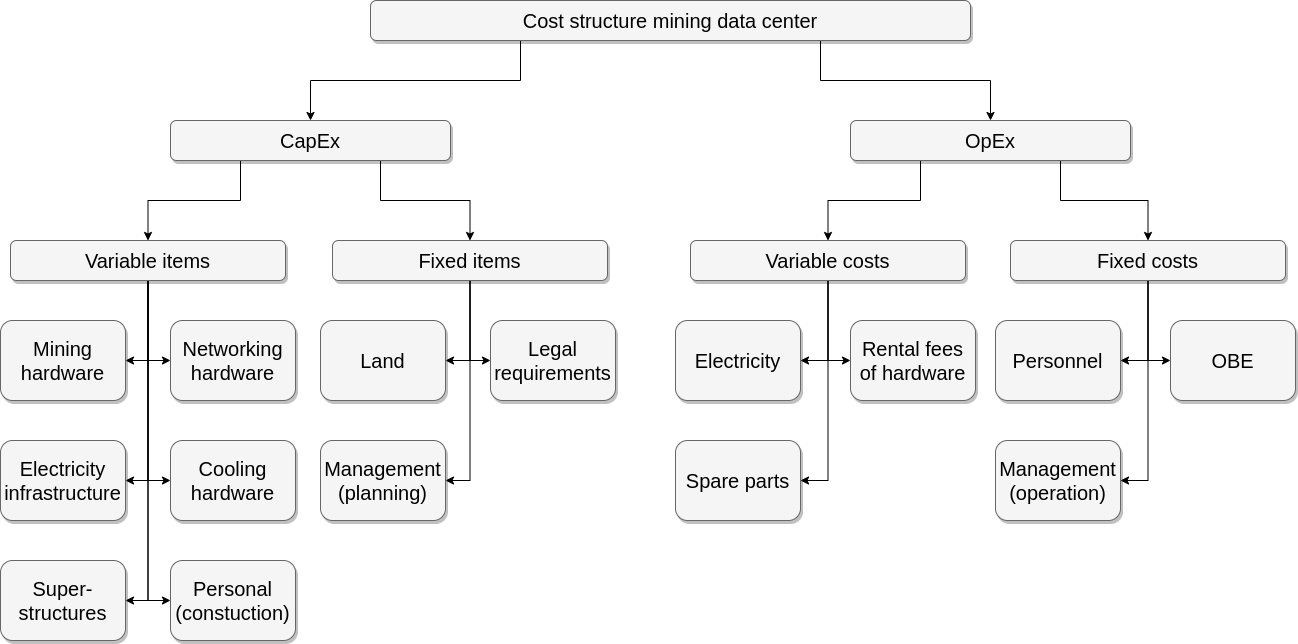
\includegraphics[width=\textwidth]{valuestructurenordics}
    \label{figure:valuestructurenordics}
\end{figure}

This division can be found in Fig. \ref{figure:valuestructurenordics}. The following items are relevant to the structure
a data center:\footcite[Cf.][]{appendix:capex}
\begin{itemize}
    \item \textbf{Mining Hardware: }This item refers to the actual special hardware that is needed for the
    Bitcoin mining (see item 2 in Fig. \ref{figure:valuechaindatacenter}). The \ac{KPI}, which measures the
    effectiveness of the device is the amount of average payouts from mining. This ranges
    for current models, such as the Antminer S19Pro, at about $0.06\ USD / \frac{TH}{s} / day$ in the worst case, means
    \ac{USD} per hashrate per day.\footcite[Cf.][]{appendix:worstcasescenario} In the most likely scenario,
    it is $0.09\ USD / \frac{TH}{s} / day$\footcite[Cf.][]{appendix:mostprobablescenario} and in the optimal scenario
    at $0.27\ USD / \frac{TH}{s} / day$.\footcite[Cf.][]{appendix:optimalscenario} The identification of the correct
    scenario is based on the Difficulty of Bitcoin mining, the total network Hashrate and the market value
    of a Bitcoin, which are additional \acp{KPI} when operating a data center. Since the market value is extremely
    volatile, it is difficult to make an accurate prediction.\footcite[Cf.][p. 325]{badertscher2017bitcoin} In addition
    this part includes the downtime and the fees for the mining pool in a lump sum
    factored in.\footcite[Cf.][]{appendix:s19proassumptions} The effectiveness of the mining hardware is
    calculated by the following equation:
    \begin{equation}
        \RM = \frac{\DP}{\THr}\cdot(1-\PF)\cdot\UT\cdot\ER
    \end{equation}
    In this formula, the daily expected payouts (\DP) per hashrate (\THr) are calculated. The result is
    corrected by uptime of the mining hardware (\UT), fees (\PF) and the exchange rate of \ac{USD} and \ac{BTC}.

    In this calculation, the electricity price is not listed directly. This value is calculated by the power consumption of the
    devices. Improvements in the firmware of these devices can be visualized with a \ac{KPI} called
    "`Reference power effiency'". This has the unit $\frac{J}{TH}$ (joules per terahash) and is strongly
    temperature dependent.\footcite[Cf.][]{s19pro2021consumption}

    The mining hardware item is variable as it is proportional to the number of miners. For a
    10MW data center, this would be approximately S19 2,987 per miner\footcite[Cf.][]{appendix:s19proassumptions} for a total price of
    of about 8,068,708 USD.\footcite[Cf.][]{appendix:capex}
    \item \textbf{Network Hardware: }In order for the mining hardware to communicate with the blockchain, network
    Hardware is required. Switches, routers and network cables fall under this item. Standardized network hardware is used
    that is cheap and available in large quantities. This item is also
    variable, as the number and length of network cabling and the number of switches increases with the number of mining hardware.
    of switches increases.\footcite[Cf.][]{appendix:capex} While the number of routers remains constant, it represents such a
    small proportion of this item that it can be considered variable. For a 10MW data center
    the cost of this item is approximately 69,060 USD.\footcite[Cf.][]{appendix:capex}
    \item \textbf{infrastructure electricity: }For the operation of the mining hardware, one item when setting up a
    of a mining data center is the power supply. This item mainly refers to the cabling within the data center.
    The grid connection and the heavy current transformers are included in other items in the invoice.
    Since the number of cables and distributors within a data center increases as the number of mining
    equipment increases, this is a variable item in the construction.\footcite[Cf.][]{appendix:capex} The cost is
    is approximately 423,900 USD for a data center with a mining power consumption of 10MW.\footcite[Cf.][]{appendix:capex}
    \item \textbf{Hardware Cooling: }As in all other data centers, cooling must be constructed on site.
    This mainly involves fans and filters that need to be installed.
    Since the number of cooling devices scales with the number of mining devices installed, this is a variable item.
    In terms of energy supply, cooling represents a constant percentage of total consumption.
    This value is primarily dependent on the climate (temperature) on site, which therefore represents a \ac{KPI}. This item
    has approximately the amount of 908,350 USD for a 10MW mining data center.\footcite[Cf.][]{appendix:capex}
    \item \textbf{Bodies: }These are primarily heavy-duty racks that are used to set up the miners.
    Also included there are other items that relate to the construction and customization of the mining data center. Since
    and the number of heavy-duty racks increase with the number of mining hardware, this part is considered a variable item.
    portion is considered a variable item. For a 10MW data center, this portion is approximately 284,850
    USD.\footcite[Cf.][]{appendix:capex}
    \item \textbf{Personnel (setup): }Initial personnel are required to set up a data center. These are
    mainly IT and electrical specialists who are hired for the construction. This part is valued at approx.
    297,321 \ac{USD} in the calculation of the \ac{CapEx}.\footcite[Cf.][]{appendix:capex} It is a variable
    item, because the larger a data center becomes the more staff is needed for a setup.\footcite[Cf.][]{appendix:capex}
    \item \textbf{Land: }This item includes the land and real estate for a mining data center. The
    financial resources required are highly dependent on the location where a data center is to be built. In the
    example calculation for the 10MW data center, which was also used in the last points, the amount of costs for this item was
    for this item was approximately 1,223,691 \ac{USD}.\footcite[Cf.][]{appendix:capex} In this case, this item is not
    designated as a variable cost, although this might seem obvious. For this reason, it is a fixed item,
    since a plot of land has a fixed size when sold. It is not possible to reduce or increase the size of a plot of land as needed.
    or increase the size of a plot of land. Therefore, this counts as a fixed item.\footcite[Cf.][]{appendix:capex}
    \item \textbf{Legal Requirements: }Depending on the country in which mining data centers are to be established, there are
    various legal requirements must be taken into account. These are primarily requirements that govern the
    operation of such a data center and the employment of personnel. Local tax law must be
    particular to be taken into account. These expenses, which largely consist of legal fees, must be taken into account even before the
    construction of a data center and occur on a one-time basis. They amount to 1,735,295 \ac{USD} if
    the example of the 10MW data center is taken as a basis.\footcite[Cf.][]{appendix:capex}
    \item \textbf{Management (planning): }Finally, \ac{CapEx} is used to calculate the initial management and cost of
    project management are calculated. These are the costs for the personnel who centrally plan such data centers and the
    associated projects. For the exemplary data center, this item amounts to approx.
    631.880 USD.\footcite[Cf.][]{appendix:capex}
\end{itemize}

By summing all the values of the previous points, it can be determined that a data center that is supposed to have a mining capacity of
of 10MW costs about 13,665,996 USD.\footcite[Cf.][]{appendix:summaryofinvestment} The distribution of the individual items
described is shown in Figure \ref{figure:capexdistribution10mw} relative to each other using the figures for a
a 10MW data center.

\begin{figure}[H]
    \caption{CapEx distribution for a 10MW data center}
    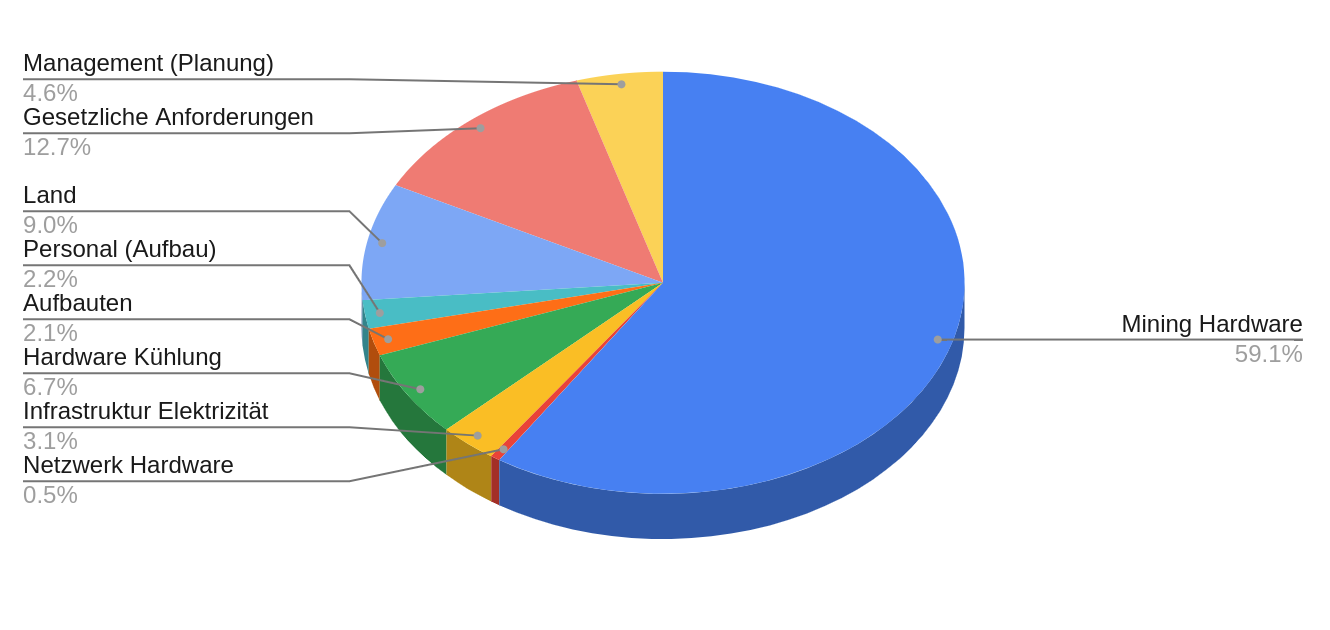
\includegraphics[width=0.7\textwidth]{capexdistribution10mw}
    \label{figure:capexdistribution10mw}
\end{figure}

In addition to the expenses that must be considered initially for a data center, the following costs (\ac{OpEx}),
which arise during operation, have to be considered:\footcite[Cf.][]{appendix:opex}
\begin{itemize}
    \item \textbf{Electricity: }This part describes the costs generated by the consumption of electricity.
    This parameter is a key component when considering \acp{KPI} of a cryptomining data center.
    (see Figure \ref{figure:valuechaindatacenter}).\footcite[Cf.][p. 327]{derks2018chaining} Since a mining data center
    is a bulk buyer from electricity, prices are subject to fluctuation, which is dictated by the provider\footcite[Cf.][]{appendix:opex}
    This item is one of the variable costs, since as the number of devices for mining and cooling increases.
    The annual cost for a 10MW data center at a base price of
    base price of $0.0357 \frac{USD}{kWh}$ circa 3,038,313 USD.\footcite[Cf.][]{appendix:opex}
    \item \textbf{Loan hardware charges: }This item carries equipment that is on loan and therefore must be paid for at regular
    periodic intervals. In the case of Genesis Group, this is the main distribution boards and transformers
    of a data center, which have a capacity greater than 1MW. Since this equipment is very expensive to purchase, it is borrowed from
    the energy suppliers. The annual cost of such a loan is about 170,280 USD for 10MW
    and are variable in nature.\footcite[Cf.][]{appendix:opex}
    \item \textbf{Spares: }In order to be able to repair defects of any hardware on site, the item of the
    spare parts is placed in the calculation for the \ac{OpEx}.\footcite[Cf.][p. 327]{derks2018chaining} For this part, there are
    no exemplary figures available.
    \item \textbf{Personnel: }To ensure that hardware can be repaired and data center operations
    can be maintained, personnel is required permanently on site. In the example, this item amounts to approx.
    31,282 USD per month, but can vary drastically from country to country.\footcite[Cf.][]{appendix:opex}
    This amount is listed under fixed costs because the initial size of the data center means that staffing plans are also
    is clear. No additional staff is hired even for small expansions.\footcite[Cf.][]{appendix:opex}
    \item \textbf{Management (Operations): }For the management of the data center and central project management, a
    flat rate of 6,289 USD per month is taken into place.\footcite[Cf.][]{appendix:opex} This describes
    the administrative costs from a central management point of view.
    \item \textbf{\ac{OBE}: }This area records the office costs, costs for the Internet, water and office electricity.
    These amount to approximately 3,593 USD per month for a 10MW data center and are fixed costs, as none of these items
    will change once the data center is up and running.\footcite[Cf.][]{appendix:opex}
\end{itemize}

\begin{figure}[H]
    \caption{OpEx distribution for a 10MW data center}
    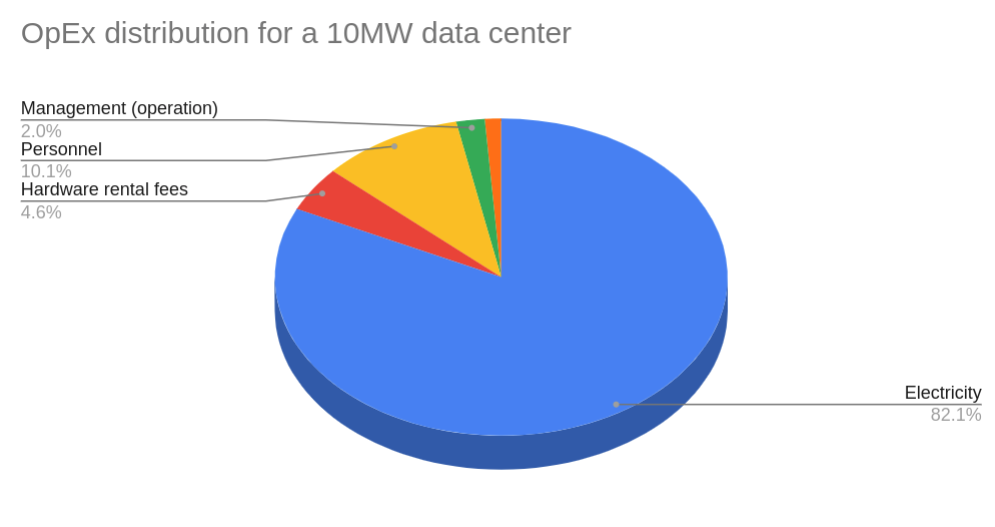
\includegraphics[width=0.7\textwidth]{opexdistribution10mw}
    \label{figure:opexdistribution10mw}
\end{figure}

In summary, for a mining capacity of 10MW, the \ac{OpEx} is approximately 317,897 USD.\footcite[Cf.][]{appendix:opex}
Now the mining has to generate revenues that amortize these expenses over time
so the company is able to make a profit. The distribution of the individual costs
is shown in Figure \ref{figure:opexdistribution10mw} relative on an annual basis.

Wie bereits in der Auszählung für \ac{CapEx} beschrieben, wird die finanzielle Effektivität eines Mining Gerätes durch
die Größe \RM betrachtet. Allerdings kann diese sehr stark fluktuieren, da dabei Faktoren, wie der Tauschkurs von Bitcoin
in USD (s. Ziffer "`Exchanges"' in Abb. \ref{figure:valuechaindatacenter}) und auch \DP, sich abhängig von den Mining
Parametern, wie Difficulty und Netzwerk Hashrate, entwickeln. Eine genaue Vorhersage ist daher nicht möglich, weshalb dort
mit verschiedenen Szenarien gerechnet wird.\footcite[Cf.][]{appendix:s19proassumptions} Aus diesen wird dann letztendlich ein
gewichteter Durchschnitt gebildet, welcher für die Kalkulation verwendet wird.\footcite[Cf.][]{appendix:s19proassumptions}

As already described in the count for \ac{CapEx}, the financial effectiveness of a mining device is
is considered by the size \RM. However, this can fluctuate greatly due to factors such as the exchange rate of Bitcoin
into USD (see figure "`Exchanges"' in Fig. \ref{figure:valuechaindatacenter}) and also \DP, vary depending on the mining
parameters, such as Difficulty and Network Hashrate. An exact prediction is therefore not possible, which is why
different scenarios are calculated.\footcite[Cf.][]{appendix:s19proassumptions} From these, a weighted average is finally formed.\footcite[Cf.][]{appendix:s19proassumptions}

\begin{figure}[H]
    \caption{Cost and value flows for a mining data center}
    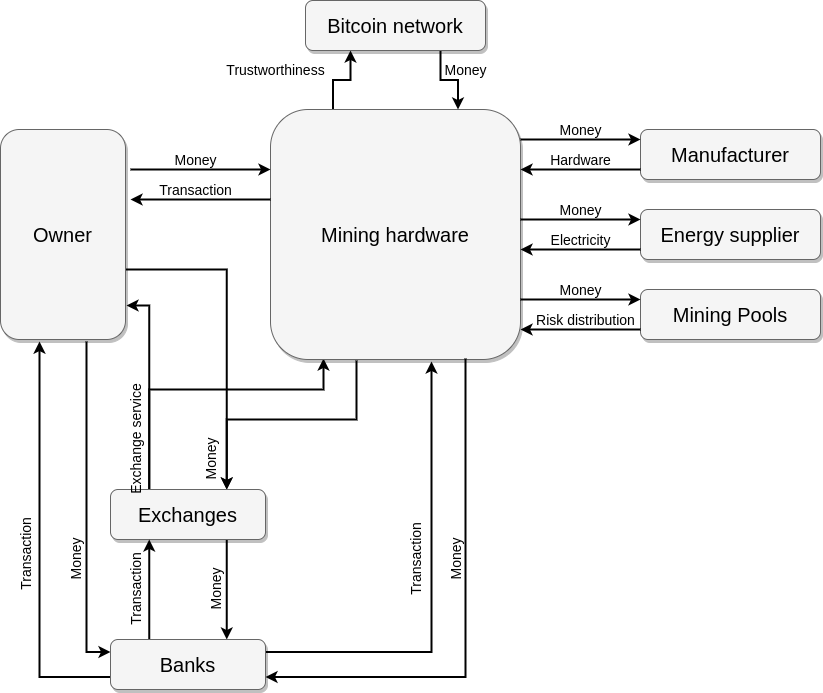
\includegraphics[width=0.7\textwidth]{valuechaindatacenter}
    \label{figure:valuechaindatacenter}
    \\
    \cite[Source: Based on][Fig. 3]{derks2018chaining}
\end{figure}

In the present example of the mining data center, the following scenarios were formed with probabilities of occurrence:

\begin{table}[H]
    \caption{Mining Effectiveness Scenarios}
    \label{tbl:miningrewardscenario}
    \begin{tabularx}{\textwidth}[ht]{X||X|X|X}
        Scenario & \RM & Probability of occurrence & Mining revenue  \\
        \hline\hline
        Worst-Case & $0,07\ USD / \frac{TH}{s} / day$ & $30\%$ & $8.224.610\frac{USD}{Year}$ \\
        \hline
        Most-Probable & $0,09\ USD / \frac{TH}{s} / day$ & $40\%$ & $10.574.499\frac{USD}{Year}$ \\
        \hline
        Optimal & $0,27\ USD / \frac{TH}{s} / day$ & $30\%$ & $31.723.497\frac{USD}{Year}$ \\
    \end{tabularx} \\
    \cite[Source: Based on][]{appendix:s19proassumptions}
\end{table}

As can be seen from table \ref{tbl:miningrewardscenario}, revenues fluctuate between 10 and over
30 million \ac{USD}, which is a considerable fuzziness. Therefore, optimization should be sought for these values.
Whether this is possible is evaluated in the following chapters. Furthermore, these calculations do not include any further
risks and will be ignored therefore. This also represents an opportunity for improvement,
since with an additional risk analysis the probabilities of occurrence can be better estimated.

Based on all financial data, cash flow and break-even point are calculable. The result of
such a calculation can be found in figure \ref{figure:datacentercashflow}. In the figure the respective values are
on an annual basis and show the development of \ac{CapEx} and \ac{OpEx} over the years.

\begin{figure}[H]
    \caption{Cash flow and break-even of a mining data center}
    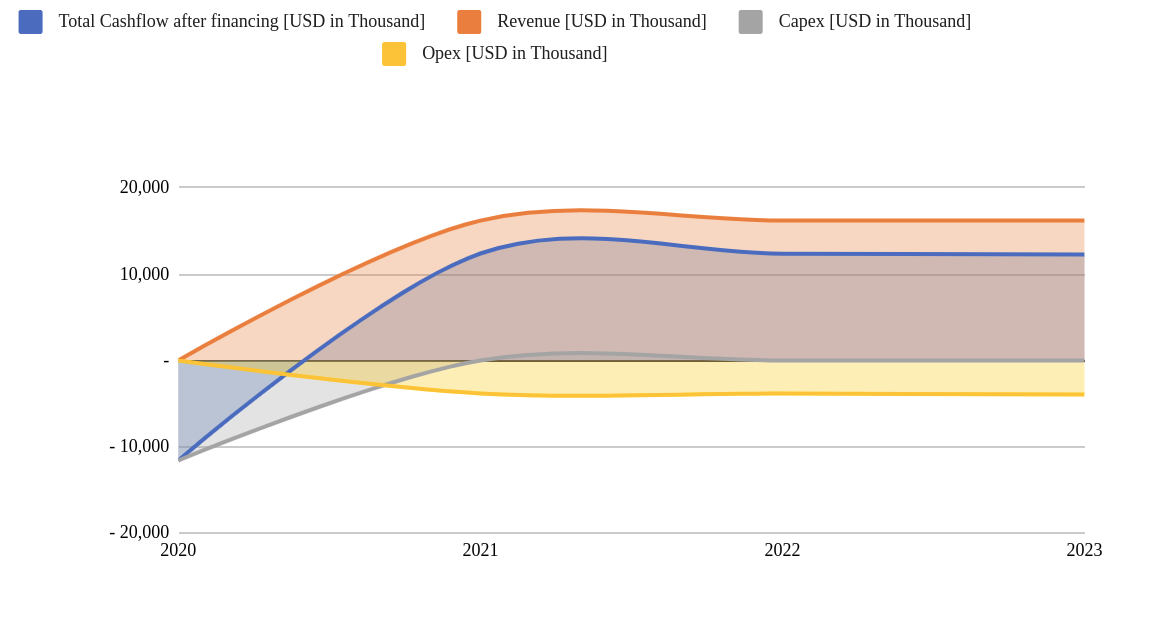
\includegraphics[width=0.7\textwidth]{datacentercashflow}
    \label{figure:datacentercashflow}
    \\
    \cite[Source: ][]{appendix:summaryofinvestment}
\end{figure}

Ultimately, there are other factors that influence the effectiveness of a data center and thus on the side of the
revenue side:
\begin{itemize}
    \item \textbf{Climate: }The climate affects the effectiveness of the miners and also significantly determines
    the dimensioning of the cooling. Accordingly, the goal in site selection is to find an optimal combination of
    electricity price, which largely determines the \ac{OpEx}, and the \ac{CapEx} for cooling, which accounts for a
    large share. However, the exact climate is not included in considerations.
    \item \textbf{Supply security: }This factor describes the security of the necessary external infrastructure,
    such as Internet and electricity. Since every failure inevitably leads to an effective complete breakdown of the data center,
    this must be included in the consideration.
\end{itemize}